% Figure: activation budgets of a reversible exterior against the horizon (thm:env-canonical(b), prop:env-horizon(a)).
% Exterior of chk:env-horizon(a): four modes with lambda(F) = (0.98, 0.9, 0.7, 0.4) in an orthonormal basis, Q = 0.5 I,
% kappa = 4 channels (no rank limit), so sigma_j(h) = |lambda_j(F)|^h = exp(-h/tau_j) with tau_j^{-1} = -ln|lambda_j(F)|
% = 0.020203, 0.105361, 0.356675, 0.916291. Solid: I_k(h) = sum_{j<k} (1/2) ln[sigma_j^2 (1 - sigma_k^2) /
% (sigma_k^2 (1 - sigma_j^2))], the budget above which variate k is read (thm:env-canonical(b)), for k = 2, 3, 4 on
% 24 points per decade of real h in [1, 100] plus the check horizons. Dashed: the linear lower bound
% h sum_{j<k} (tau_k^{-1} - tau_j^{-1}) of prop:env-horizon(a), slopes 0.085158, 0.58779, 2.26663; the gap
% I_2 - bound is 0.784, 0.486, 0.0089 at h = 1, 10, 100. Recomputed in double precision: the singular values of the
% whitened cross-covariance P0^{-1/2} P0 (F^h)^T P0^{-1/2} of a random orthonormal realization (detailed balance to
% 9e-16) equal |lambda(F)|^h to 4e-8 relative for all four at h <= 20, and the I_2, I_3 they give at h = 40, 80 equal
% the closed form to four decimals (sigma_4 is below double-precision resolution there); water-filling with the
% water level found by bisection reads k - 1 variates just below I_k(h) and k just above it. Dots: I_2 = 0.8693,
% 0.9145, 1.0607, 1.3375, 1.9907, 3.5169, 6.8328 at h = 1, 2, 5, 10, 20, 40, 80, the values printed in
% chk:env-horizon(a). Dotted: fixed budgets of 1.5, 3 and 6 nats. At 1.5 nats I_2(h) = 1.5 at h = 12.664 (two
% variates for h <= 12, one from h = 13) and the bound reaches 1.5 at the sufficient horizon
% 1.5/(tau_2^{-1} - tau_1^{-1}) = 17.614 (circles). At 3 nats the count falls 3, 2, 1 at h = 2.746, 33.477; at 6 nats
% it falls 4, 3, 2, 1 at h = 1.748, 9.069, 70.101. I_3(1) = 2.3593 > 1.5, so a third variate is never read at 1.5 nats.
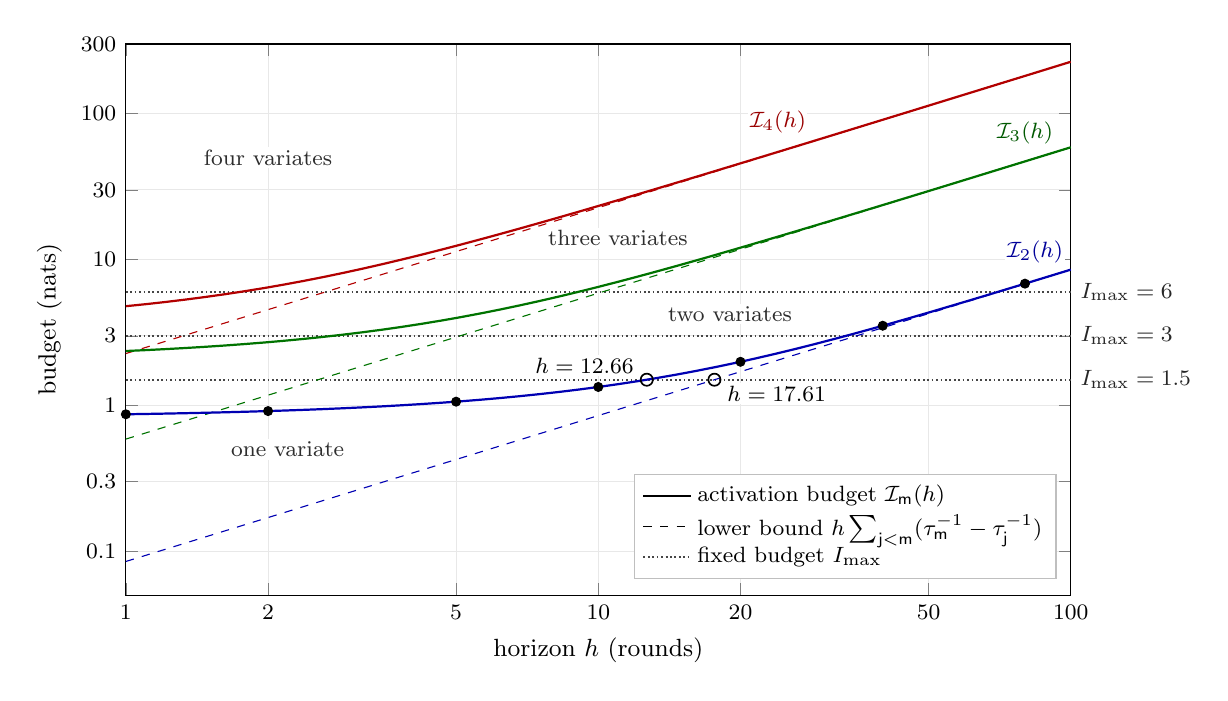
\begin{tikzpicture}
  \begin{axis}[width=12.0cm, height=7cm, scale only axis, xmode=log, ymode=log,
      xmin=1, xmax=100, ymin=0.05, ymax=300,
      xtick={1,2,5,10,20,50,100}, ytick={0.1,0.3,1,3,10,30,100,300}, log ticks with fixed point,
      grid=major, grid style={gray!18}, clip=false,
      xlabel={horizon $h$ (rounds)}, ylabel={budget (nats)},
      every axis label/.style={font=\small}, tick label style={font=\footnotesize},
      legend style={font=\footnotesize, at={(0.985,0.03)}, anchor=south east, draw=gray!50, fill=white,
        cells={anchor=west}, row sep=-1pt}]
    % fixed budgets
    \draw[gray!55!black, densely dotted, semithick] (axis cs:1,1.5) -- (axis cs:100,1.5);
    \draw[gray!55!black, densely dotted, semithick] (axis cs:1,3) -- (axis cs:100,3);
    \draw[gray!55!black, densely dotted, semithick] (axis cs:1,6) -- (axis cs:100,6);
    % linear lower bounds of prop:env-horizon(a), straight lines on these axes
    \addplot[blue!70!black, dashed, forget plot] coordinates {(1,0.085158) (100,8.5158)};
    \addplot[green!45!black, dashed, forget plot] coordinates {(1,0.58779) (100,58.779)};
    \addplot[red!70!black, dashed, forget plot] coordinates {(1,2.2666) (100,226.66)};
    % activation budgets I_2, I_3, I_4
    \addplot[blue!70!black, thick, forget plot] coordinates {(1,0.86926) (1.1007,0.87373) (1.2115,0.87868) (1.3335,0.88415) (1.4678,0.8902) (1.6156,0.8969) (1.7783,0.90432) (1.9573,0.91254) (2,0.9145) (2.1544,0.92165) (2.3714,0.93176) (2.6102,0.94298) (2.873,0.95545) (3.1623,0.96931) (3.4807,0.98474) (3.8312,1.0019) (4.217,1.0211) (4.6416,1.0425) (5,1.0607) (5.109,1.0663) (5.6234,1.0931) (6.1897,1.123) (6.8129,1.1565) (7.4989,1.1942) (8.254,1.2364) (9.0852,1.284) (10,1.3375) (11.007,1.3978) (12.115,1.4657) (13.335,1.5424) (14.678,1.6289) (16.156,1.7265) (17.783,1.8366) (19.573,1.9607) (20,1.9907) (21.544,2.1006) (23.714,2.2579) (26.102,2.4348) (28.73,2.6333) (31.623,2.8556) (34.807,3.1043) (38.312,3.382) (40,3.5169) (42.17,3.6914) (46.416,4.0358) (51.09,4.4185) (56.234,4.8432) (61.897,5.3138) (68.129,5.8347) (74.989,6.4107) (80,6.8328) (82.54,7.0471) (90.852,7.7496) (100,8.5247)};
    \addplot[green!45!black, thick, forget plot] coordinates {(1,2.3593) (1.1007,2.3931) (1.2115,2.4308) (1.3335,2.4729) (1.4678,2.5198) (1.6156,2.5723) (1.7783,2.631) (1.9573,2.6968) (2,2.7126) (2.1544,2.7705) (2.3714,2.8533) (2.6102,2.9463) (2.873,3.0509) (3.1623,3.1687) (3.4807,3.3014) (3.8312,3.451) (4.217,3.6197) (4.6416,3.81) (5,3.974) (5.109,4.0245) (5.6234,4.2662) (6.1897,4.5385) (6.8129,4.8449) (7.4989,5.1892) (8.254,5.5755) (9.0852,6.0084) (10,6.4926) (11.007,7.0333) (12.115,7.6361) (13.335,8.3071) (14.678,9.0529) (16.156,9.8808) (17.783,10.799) (19.573,11.815) (20,12.058) (21.544,12.94) (23.714,14.184) (26.102,15.558) (28.73,17.076) (31.623,18.751) (34.807,20.6) (38.312,22.639) (40,23.622) (42.17,24.887) (46.416,27.366) (51.09,30.098) (56.234,33.108) (61.897,36.425) (68.129,40.078) (74.989,44.103) (80,47.043) (82.54,48.534) (90.852,53.414) (100,58.788)};
    \addplot[red!70!black, thick, forget plot] coordinates {(1,4.7866) (1.1007,4.9402) (1.2115,5.113) (1.3335,5.3076) (1.4678,5.527) (1.6156,5.7742) (1.7783,6.053) (1.9573,6.3673) (2,6.4432) (2.1544,6.7215) (2.3714,7.1203) (2.6102,7.569) (2.873,8.0733) (3.1623,8.6392) (3.4807,9.2732) (3.8312,9.9825) (4.217,10.775) (4.6416,11.658) (5,12.411) (5.109,12.641) (5.6234,13.734) (6.1897,14.948) (6.8129,16.294) (7.4989,17.786) (8.254,19.437) (9.0852,21.263) (10,23.282) (11.007,25.513) (12.115,27.976) (13.335,30.695) (14.678,33.695) (16.156,37.004) (17.783,40.653) (19.573,44.676) (20,45.635) (21.544,49.11) (23.714,53.996) (26.102,59.379) (28.73,65.309) (31.623,71.841) (34.807,79.036) (38.312,86.959) (40,90.776) (42.17,95.684) (46.416,105.29) (51.09,115.87) (56.234,127.52) (61.897,140.34) (68.129,154.46) (74.989,170) (80,181.35) (82.54,187.11) (90.852,205.94) (100,226.67)};
    % values of chk:env-horizon(a) on I_2
    \addplot[only marks, mark=*, mark size=1.6pt, black, forget plot] coordinates {(1,0.8693) (2,0.9145) (5,1.0607) (10,1.3375) (20,1.9907) (40,3.5169) (80,6.8328)};
    % budget 1.5: I_2 reaches it at h = 12.664, the bound at the sufficient horizon 17.614
    \addplot[only marks, mark=o, mark size=2.2pt, black, semithick, forget plot] coordinates {(12.664,1.5) (17.614,1.5)};
    \node[font=\footnotesize, anchor=south east, inner sep=1pt, fill=white, xshift=-3.5pt, yshift=1pt] at (axis cs:12.664,1.5) {$h=12.66$};
    \node[font=\footnotesize, anchor=north west, inner sep=1pt, fill=white, xshift=3.5pt, yshift=-1pt] at (axis cs:17.614,1.5) {$h=17.61$};
    % curve labels
    \node[font=\footnotesize, blue!60!black, inner sep=0.5pt, fill=white] at (axis cs:84,11.2) {$\mathcal I_2(h)$};
    \node[font=\footnotesize, green!35!black, inner sep=0.5pt, fill=white] at (axis cs:80,74) {$\mathcal I_3(h)$};
    \node[font=\footnotesize, red!60!black, inner sep=0.5pt, fill=white] at (axis cs:24,88) {$\mathcal I_4(h)$};
    % regions: number of variates read at a budget in the region
    \node[font=\footnotesize, gray!35!black, inner sep=1pt, fill=white] at (axis cs:2.2,0.5) {one variate};
    \node[font=\footnotesize, gray!35!black, inner sep=1pt, fill=white] at (axis cs:19,4.24) {two variates};
    \node[font=\footnotesize, gray!35!black, inner sep=1pt, fill=white] at (axis cs:11,14) {three variates};
    \node[font=\footnotesize, gray!35!black, inner sep=1pt, fill=white] at (axis cs:2,50) {four variates};
    % budget labels outside the frame
    \node[font=\footnotesize, gray!30!black, anchor=west] at (axis cs:100,1.5) {$I_{\max}=1.5$};
    \node[font=\footnotesize, gray!30!black, anchor=west] at (axis cs:100,3) {$I_{\max}=3$};
    \node[font=\footnotesize, gray!30!black, anchor=west] at (axis cs:100,6) {$I_{\max}=6$};
    % legend of line styles
    \addlegendimage{black, thick}
    \addlegendentry{activation budget $\mathcal I_{\mathsf m}(h)$}
    \addlegendimage{black, dashed}
    \addlegendentry{lower bound $h\sum_{\mathsf j<\mathsf m}(\tau_{\mathsf m}^{-1}-\tau_{\mathsf j}^{-1})$}
    \addlegendimage{gray!55!black, densely dotted, semithick}
    \addlegendentry{fixed budget $I_{\max}$}
  \end{axis}
\end{tikzpicture}
